\begin{figure}[tbh]
	\centering
	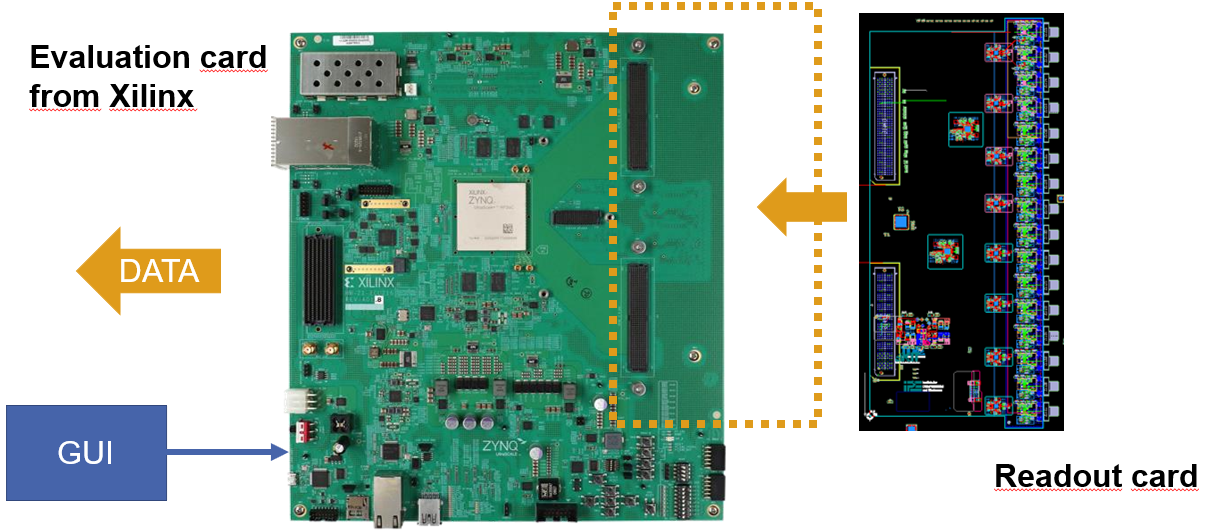
\includegraphics[width = \textwidth]{chap/04-work/img/concept_theresa}
	\caption{General concept of the new readout system}
	\label{fig:concept_theresa}
\end{figure}

\section{Optical part}
\section{Front-End Card}
\autoref{fig:theresa_scheme} shows the general schema of the sampling system, reduced to four channels for presentation purposes.
\begin{figure}[H]
	\centering
	\includegraphics[width = \textwidth]{chap/04-work/img/theresa_scheme.tikz}
	\caption{Placeholder: General schema of THERESA. For presentation purposes only four channels are shown.}
	\label{fig:theresa_scheme}
\end{figure}

\section{Readout Card}
\section{Selection Of The Card}\label{sec:selection}
When selecting the Readout Card, following criteria need to be considered:
\begin{itemize}
	\item Integrated \glspl{adc}
	\item Number, resolution and bandwidth of \glspl{adc}
	\item Peripheral connections
	\item Flexibility/Customization
	\item Suitable connectivity for high-data-throughput
\end{itemize}


\begin{figure}[tbh]
	\centering
	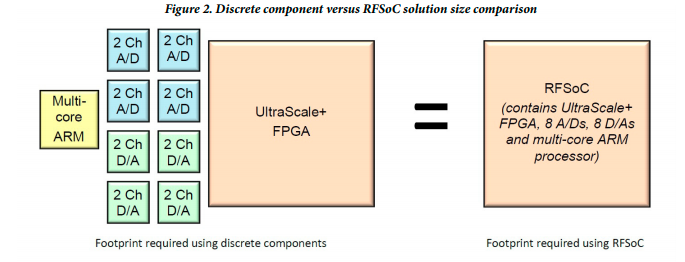
\includegraphics[width = \textwidth]{chap/04-work/img/footprint}
	\caption{Placeholder: Discrete vs IC}
	\label{fig:footprint}
\end{figure}